\chapter{Methods}

While the self-supervised denoising methods discussed so far eliminate the need for clean data, most still require large datasets of noisy images or are limited to specific noise types.
A notable exception is the Deep Image Prior (DIP) introduced by Ulyanov~et al.~\cite{DIP}.
DIP is a zero-shot method, meaning it operates on a single noisy sample, and does not make any explicit assumptions about the noise distribution.

In this chapter, we present DIP and its various extensions.
First, we describe the fundamental principles of DIP, followed by common techniques used to further regularize the solution.
Finally, we explore additional DIP-based approaches that build upon these foundations.

\section{Deep Image Prior}

As discussed in Section~\ref{sec:denoising}, denoising is an ill-posed inverse problem and therefore appropriate regularization is crucial in order to obtain plausible solutions.
This is typically expressed as an optimization problem of the form
\begin{equation}\label{eq:ip-optim}
    \hat{x} = \argmin_x L(x,y) + R(x),
\end{equation}
where $L(x,y)$ is a data fidelity term that ensures that the denoised estimate $\hat{x}$ stays close to the noisy signal $y$ and $R(x)$ is the regularizer.
Most traditional, non-deep-learning methods, such as total variation denoising~\cite{TV}, rely on an explicit regularization term.
The self-supervised methods discussed in Section~\ref{sec:self-supervised} do not necessarily include such a term; however, they do make specific assumptions about the solution (e.g., zero-mean or spatially independent noise), which are implicitly encoded in the training procedure --- through techniques like sub-sampling or masking.

In contrast, DIP does not make any explicit assumptions about the noise or image structure.
Instead, it relies solely on the architecture of a convolutional neural network to implicitly regularize the solution.
The key idea is to parameterize an image $x$ as the output of an CNN $f_\theta$ through $x = f_\theta(z)$, where $z$ refers to a random vector, e.g., $z \sim \normal$.
\begin{figure}
    \centering
    \begin{tikzpicture}[scale=1.5]
        \useasboundingbox (-3,3.5) rectangle (3,-0.5);

        % Coords
        \coordinate (t0) at (1,3.5);
        \coordinate (t1) at (-0.2,3.3);
        \coordinate (t2) at (-1.4,2.9);
        \coordinate (t3) at (-2.4,2);
        \coordinate (t4) at (-2.2,0.8);
        \coordinate (t5) at (-1,0.2);
        \coordinate (x) at (-1.8,1.8);
        \coordinate (y) at (0,0);
        \coordinate (p) at (-0.6,0.6);

        % Curves
        \draw[very thick, RoyalBlue, dashed] (x) -- (y);
        \draw[very thick, black, -{Latex[length=8pt,width=8pt]}, shorten >=4pt] plot [smooth, tension=0.7] coordinates {(t0) (t1) (t2) (t3) (t4) (t5) (y)};
        \draw[very thick, JungleGreen, -{Latex[length=8pt,width=8pt]}, shorten >=4pt] (t0) to[out=-80, in=10] (p);
        \draw[very thick, Orchid, -{Latex[length=8pt,width=8pt]}, shorten >=4pt] (t0) .. controls (4,2) and (3,0.5) .. (y);

        % Points
        \fill[black] (t0) circle (2pt);
        \fill[black] (t1) circle (2pt);
        \fill[black] (t2) circle (2pt);
        \fill[Maroon] (t3) circle (2pt);
        \fill[black] (t4) circle (2pt);
        \fill[black] (t5) circle (2pt);
        \fill[RoyalBlue] (x) circle (2pt);
        \fill[RoyalBlue] (y) circle (2pt);

        % Labels
        \node[above, yshift=2pt] at (t0) {$t_0$};
        \node[above, yshift=2pt] at (t1) {$t_1$};
        \node[above, yshift=2pt] at (t2) {$t_2$};
        \node[left, xshift=-2pt, Maroon] at (t3) {$t_3$};
        \node[left, xshift=-2pt] at (t4) {$t_4$};
        \node[below, yshift=-2pt] at (t5) {$t_5$};
        \node[below, yshift=-2pt, RoyalBlue] at (x) {$x$};
        \node[below, yshift=-2pt, RoyalBlue] at (y) {$y$};

        \node[below] at (-0.8, 3) {\sffamily DIP};
        \node[below, JungleGreen, align=center] at (1.7,2) {\sffamily Conventional\\prior};
        \node[below, Orchid] at (2,0.3) {\sffamily No prior};
    \end{tikzpicture}
    \caption{
        The effect of priors.
        Without regularization, the optimization leads directly to the noisy image $y$.
        Conventional priors shift the solution closer to the clean image $x$.
        DIP will eventually overfit to $y$, but often the optimization path will pass close to $x$, with the optimal stopping point marked in red.
        Figure adapted from~\cite{DIP}.
    }\label{fig:priors}
\end{figure}
This means that instead of optimizing $x$ directly, the reconstruction is constrained by the network's ability to map $z$ to a plausible image.
In terms of (\ref{eq:ip-optim}), the MSE is used as the loss function and the regularizer $R(x)$ is replaced with the implicit prior induced by the network structure, leading to the following optimization:
\begin{equation}
    \theta^* = \argmin_\theta \norm{f_\theta(z) - y}_2^2.
\end{equation}
After training the network using gradient descent, the denoised estimate is then obtained as $\hat{x} = f_{\theta^*}(z)$.
The random vector $z$ remains fixed throughout the training process.
The regularizing effect of this parametrization relies on the observation that CNNs tend to capture structured patterns (e.g., edges and textures) before fitting to high-frequency noise.
However, since the network is sufficiently expressive, it will eventually memorize the noise, leading to overfitting.
Thus, it is crucial to identify the optimal stopping point, at which the network successfully learned the underlying image structure while minimizing the influence of noise.
This process is visualized in Figure~\ref{fig:priors}.
Formally, this regularizer can be expressed as
\begin{equation}
    R(x) = \begin{cases}
        0 &\text{$f_\theta$ can produce $x$ in $N$ steps}\\
        +\infty &\text{else}
    \end{cases}
\end{equation}
where $N$ refers to a fixed maximum number of iterations.
However, such a fixed stopping point is not ideal because the optimal stopping point depends on factors such as the specific image $x$, the random vector $z$ and also the initial network parameters $\theta_0$.

\subsection{Early Stopping}

\begin{figure}[t]
    \centering
    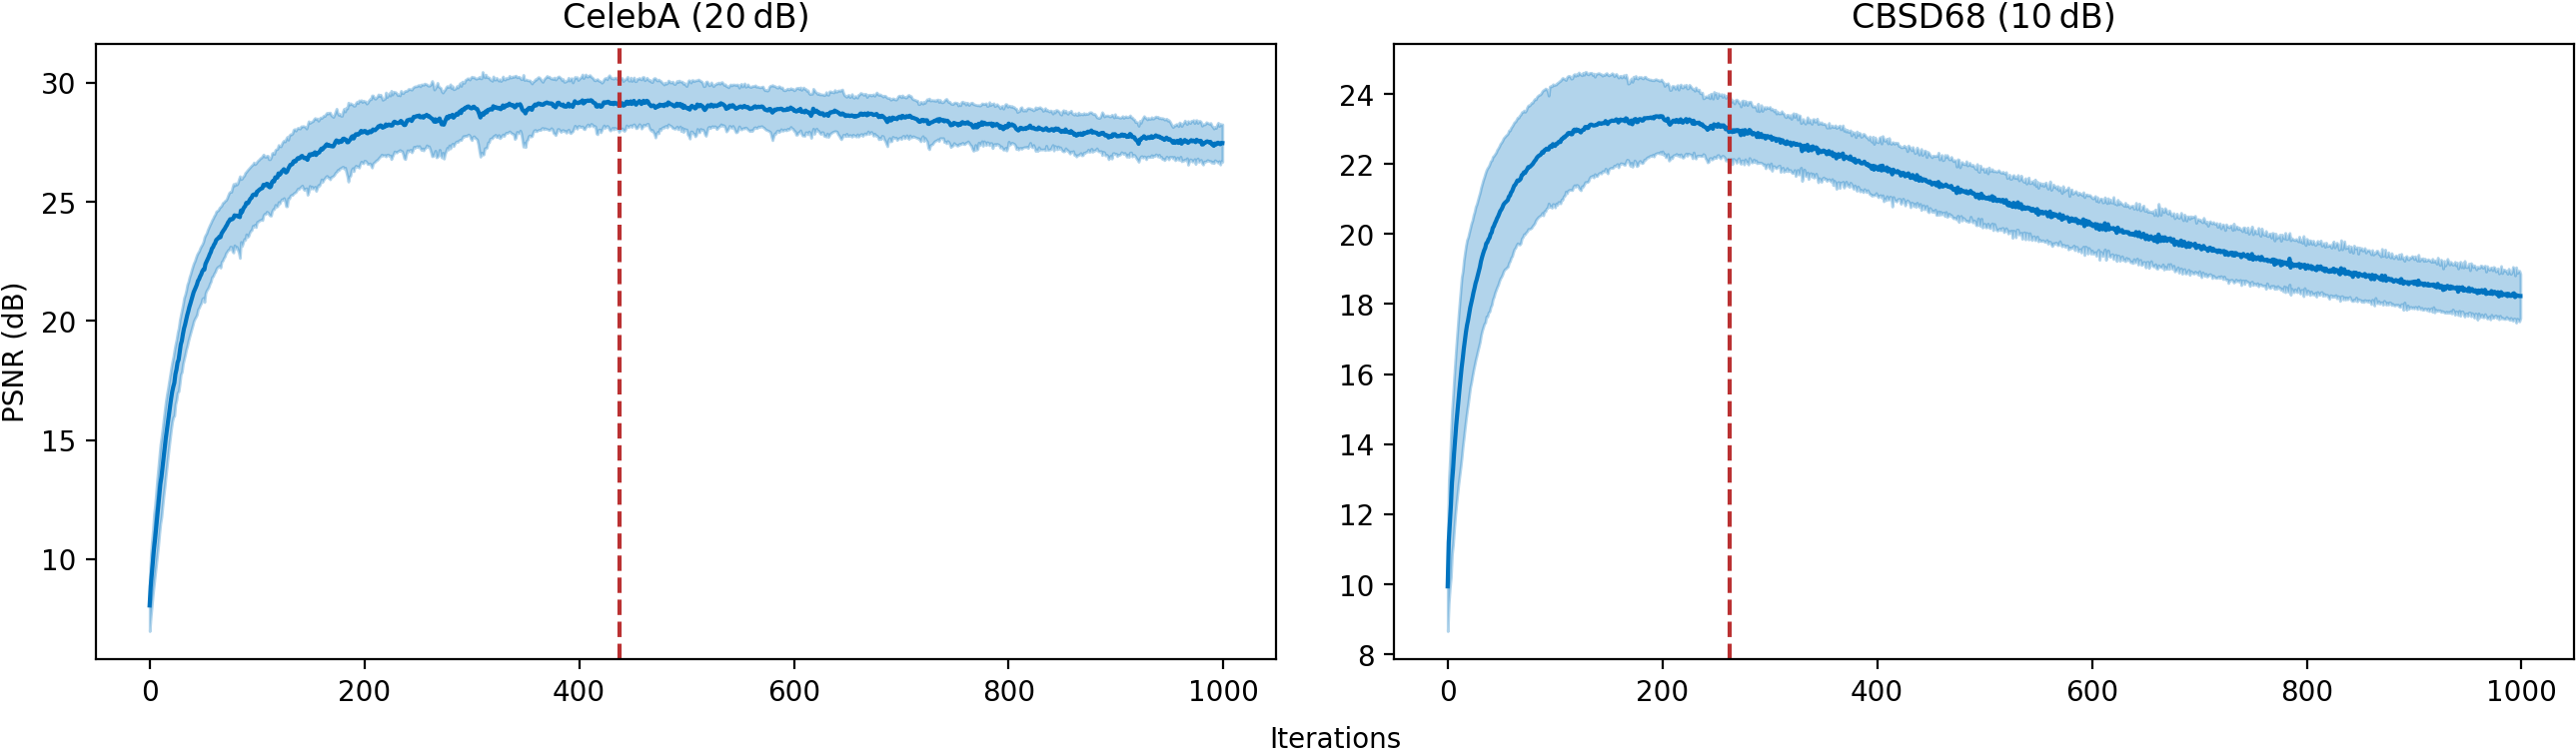
\includegraphics[width=\textwidth]{img/fig_4.2.png}
    \caption{
        ES-WMV on different datasets and noise levels.
        Image quality is evaluated on 20 random images from the CelebA (left) and CBSD68 (right) datasets, with Gaussian noise added at levels specified in the titles.
        The blue line represents the mean PSNR, the light blue shaded area indicates ±1 standard deviation.
        The red line marks the average detected stopping point.
    }\label{fig:early-stopping}
\end{figure}

The process of halting the training to mitigate overfitting is known as early stopping (ES).
As discussed earlier, a fixed stopping point generally will not work well.
Therefore, we need to find a way to dynamically detect optimal stopping points during training.
In principle, if the clean ground-truth image $x$ were available, this would be trivial:
One could simply track image quality using an appropriate metric, e.g., PSNR or SSIM, and stop training at its peak.
However, since $x$ is inherently unknown in the denoising setting, we need an alternative criterion to determine when to stop.

Wang et al.~\cite{ES} propose such a criterion based on the running variance of the DIP reconstructions over time.
Let $\{x^t\}_{t \geq 1}$ denote the sequence of the respective denoised estimates $x^t = f_{\theta^t}(z)$ at iteration $t$.
The authors observe that the MSE $\norm{x^t-x}_F^2$ initially drops as the networks learns the image structure, and then rises again due to overfitting to noise, leading to a U-shaped curve.
However, once again, $x$ is unknown in practice, so the goal is to detect the minimum of said curve without access to $x$.
To achieve this, they consider the running variance over a window of $W$ iterations, given by
\begin{equation}\label{eq:VAR}
    \Var(t) = \frac{1}{W} \sum_{w=0}^{W-1} \norm[\Big]{x^{t+w}-\frac{1}{W} \sum_{i=0}^{W-1} x^{t+i}}_F^2.
\end{equation}
Intuitively, when $t$ is near the optimal stopping point, all $x^t$'s should be close to $x$, leading to $\frac{1}{W} \sum_{w=0}^{W} x^t \approx x$.
Plugging this back into~(\ref{eq:VAR}), we see that when $t$ is near the optimum, $\Var(t)$ approximates the average MSE across the window.
Therefore, they propose using the minimum of the variance curve to determine the stopping point.
To improve robustness, they introduce a patience parameter $P$, allowing the variance to stagnate for up to $P$ iterations before stopping.
This approach, termed early stopping via windowed moving variance (ES-WMV), is effective across different noise levels and types of images, as demonstrated in Figure~\ref{fig:early-stopping}. 

\subsection{Total Variation}

Another way to prevent overfitting is to incorporate an additional explicit regularization term, such as total variation (TV)~\cite{TV}.
TV encourages piecewise smoothness by penalizing abrupt intensity changes in the image.
Formally, for an image $x \in \R^{m \times n}$, it is defined as
\begin{equation}
    \text{TV}(x) = \sum_{i=1}^{m-1} \sum_{j=1}^{n-1} (|x_{i+1,j} - x_{i,j}| + |x_{i,j+1} - x_{i,j}|).
\end{equation}
Liu et al.\ propose combining the implicit network regularization of DIP with an explicit TV regularizer, leading to the method known as DIP-TV~\cite{DIP-TV}. This results in the following optimization problem:
\begin{equation}
    \theta^* = \argmin_\theta \norm{f_\theta(z) - y}_2^2 + \lambda \text{TV}(f_\theta(z)).
\end{equation}

\section{Deep Diffusion Image Prior}


\section{Self-Guided Deep Image Prior}
